\clearpage
\chapter{\textbf{Stand der Technik für Anwesenheitserkennung/-Prognose}}\label{grundlagen}
%\addtocontents{toc}{\vspace{0.5cm}}

Man kann verschiedene Techniken zur Anwesenheitserkennung und -Prognose in Innenräumen in \text{aktive} und
\textit{passive} Verfahren unterteilen. \\\\
%\section{Aktive und Passive Messverfahren}
Aktive Verfahren messen die menschliche Anwesenheit etwa mit 
Kamera- oder Infrarotsensoren, welche den Menschen direkt im Raum erkennen können. Ein Kamerasensor nimmt
dabei kontinuierlich Bilder des Raumes auf, während ein Algorithmus im Hintergrund versucht ein 3D-Modell 
eines menschlichen Skeletts auf sich bewegende Teile des Bildes zu legen. Bewegen sich über mehrere Bilder 
hinweg die Bereiche auf und unmittelbar neben dem 3D-Modell, registriert das System eine Anwesenheit.\\\\
Infrarotsensoren dagegen funktionieren eher wie ein klassischer Bewegungsmelder, welcher Unterschiede in der 
Infrarotstrahlung eines Raumes erkennt. Durch die generierte Körperwärme des menschlichen Körpers, sorgt ein
Mensch, der sich durch den Sensor bewegt, für einen Ausschlag des Sensors.\\

Passive Verfahren orientieren sich an den physikalischen Eigenschaften des Raumes. Anstatt die Präsenz des 
Menschen direkt zu messen, wird versucht, diese von Veränderungen der Eigenschaften der Raumluft oder 
elektromagnetischer Strahlung des Raumes zu erkennen. \\
Verändert sich beispielsweise durch menschliche Anwesenheit die Luftfeuchtigkeit 
in einem Raum in sehr geringem Maß, wird die  Laufzeit einer Ultraschallwelle die durch diesen Raum 
geschickt wird, leicht verringert, da die Schallgeschwindigkeit in dichteren Medien zunimmt.\\
Die Systeme unterscheiden sich neben der Art der Messung auch deutlich in der Komplexität der Implementierung.
Während Ultraschallsensoren wegen der verhätlnismäßig geringen Schallgeschwindigkeit keine besonders hohe 
Genauigkeit besitzen müssen, sind die an einen Mikrowellensensor gestellten Ansprüche wesentlich höher, da sich
Mikrowellen mit $300\cdot10^6 \,m/s$ gegenüber der Schallgeschwindigkeit mit lediglich etwa $330\, m/s$ ausbreiten.
Mit Mikrowellen können Bewegungen durch Ausnutzung des Doppler-Effektes einer elektromagnetischen Welle erkannt 
werden. Bewegen sich Objekte oder Personen auf den Sensor zu, wird das Echo der Welle gestaucht, wodurch die 
Bewegung erkannt wird.\\
Hier verdeutlicht sich nochmals die Motivation dieser Arbeit, da Sensoren für Temperatur, Luftfeuchtigkeit, oder CO2
weder teuer sind, noch besondere Ansprüche an Positionierung im Raum oder Kallibrierung besitzen.

\chapter{\textbf{Untersuchte Verfahren}}

\section{Machine Learning}\label{unterkapitel}
\addtocontents{toc}{}%\vspace{0.8cm}}

Machine Learning ist ein Teilbereich der künstlichen Intelligenz und beschreibt das Entwickeln mathematischer 
Modelle zur statistischen Auswertung von Daten.\\
Dabei wird dem Modell anhand von Trainigsdaten beigebracht, Gesetzmäßigkeiten zu erkennen, um danach Erwartungen 
über bisher unbekannte Daten treffen zu können.  
Beispielsweise könnte ein solches Modell aus einem Datenset mit der aktuellen Jahreszeit, Uhrzeit und 
Position der Sonne am Himmel trainiert werden, sodass es auch schließlich in einem anderen Datenset 
aus Jahreszeit und Position der Sonne Rückschlüsse auf die Uhrzeit treffen kann.\\
Als Vorbild für diesen ,,Lernvorgang'' dient das menschliche Gehirn, welches ebenfalls versucht zwischen 
bestimmten Input-Parametern wie z.B. der Form und Farbe eines Gegenstandes eine Beziehung herzustellen,
um das beobachtete Objekt in Zukunft schneller kategorisieren zu können.\\
Da eine Vielzahl von effektiven Machine Learning Algorithmen existiert, ist es essenziell, sich mit den
Stärken und Schwächen einzelner Herangehensweisen zu befassen.\\

In dieser Arbeit sollen zwei Unterkategorien des Machine Learning genauer betrachtet werden:
\begin{itemize}
    \item \textit{Supervised Learning} 
    \item \textit{Unsupervised Learning}
\end{itemize}
\textit{Supervised Learning} bedeutet zwischen bestimmten Feldern eines Datensets eine Beziehung
zu einem sog. Label herzustellen, welches als eine Art Ergebnis aus den Eingabewerten gesehen 
werden kann. Ein so traniertes Model kann dann neue, ihm vorher unbekannte Datensets, mit einem 
Label versehen - etwa wie in dem o.g. Beispiel wo Jahreszeit und Sonnenposition die Eingabewerte 
und die Uhrzeit das Label darstellen. Der Begriff ,,\textit{supervised}'' ergibt sich daraus, dass 
das Datenset, mit dem das Model traniert wird, diese Labels gegeben 
hat, sodass das Modell sich bei jedem Schritt des Lernvorgangs selbst korrigieren kann, falls 
eine Fehleinschätzung getroffen wurde.
Bei einer sog. ,,\textit{Klassifizierung}'' sind diese Labels fest vorgegeben, während sie in der 
,,\textit{Regression}'' kontinuierlicher Natur sind. Im Kontext dieser Arbeit wäre das Ergebnis einer 
Klassifizierung eine ,,1'' für Anwesenheit und eine ,,0'' für Abwesenheit, während das Ergebnis einer 
Regression eine Wahrscheinlichkeit auf Anwesenheit zwischen 0.0 und 1.0 darstellen würde.
\newpage
Beim ,,\textit{Unsupervised Learning}'' versucht das Modell ohne Referenz zu einem bestimmten 
Label, Zusammenhänge zwischen bestimmten Feldern des Datensets herzustellen. Solche Modelle 
arbeiten vorrangig mit ,,\textit{Clustering}'' und ,,\textit{Dimensionality Reduction}''.\\
,,\textit{Clustering}''-Algorithmen versuchen ein Datenset in kleinere Teilmengen einzuteilen und
so aus den Feldern des Datensets bestimmte Abhängigkeiten abzuleiten.

\begin{figure}[h]
    \centering
    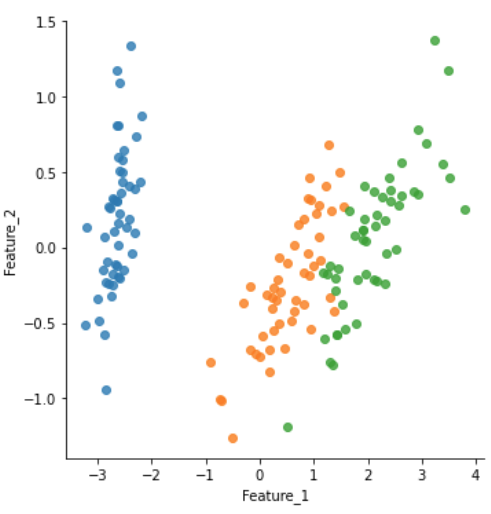
\includegraphics[width=8.0cm]{./pic/Clustering_Beispiel.png}
    \caption{Beispiel für Clustering}
    \label{fig:Clustering_Beispiel}
\end{figure}

Bei der ,,\textit{Dimensionality Reduction}'' versucht der Algorithmus das Datenset in seiner 
Dimensionalität, also seiner Anzahl an Feldern, zu reduzieren. Es wird also die Frage gestellt, 
ob sich in einem bestehenden Datenset auch mit weniger Feldern Abhängigkeiten feststellen lassen. Dieser 
Schritt wird vorallem für Modelle benutzt, die sensibel gegenüber hoher Dimensionalitäten sind, 
sodass das Datenset vor dem Training in seiner Dimensionalität heruntergebrochen werden kann.

Im Rahmen des Projektes wurden hauptsächlich Klassifizierungs-Algorithmen genutzt, da ein Großteil der 
Datensets Labels zur Überprüfung hatte.\\
Um einen Vergleich herzustellen werden später trotzdem noch 
einzelne Ergebnisse von Clustering und Dimensionality Reduction betrachtet. Im Folgenden sollen die genutzten 
Modelle erklärt werden.
\newpage
\subsection{Random Forest Classifier}

\textit{Random Forest Classifier} RFC stellen eine Unterkategorien der ,,\textit{Decision Trees}'' dar. Decision Trees sind einfache
Anordnungen von bestimmten Fragen, die über das Datenset gestellt werden, um eine Klassifikation zu erreichen.

\begin{figure}[h]
    \centering
    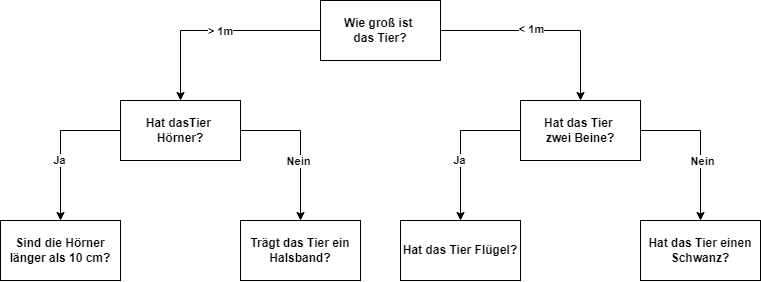
\includegraphics[width=10.0cm]{pic/DecisionTree.png}
    \caption{Beispiel eines Decision Trees}
    \label{fig:DT_Beispiel}
\end{figure}

Erstellt man ein ,,\textit{Ensemble}'' aus Decision Trees die Erwartungen über einen zufällig gewählten 
Teil des Datensets treffen können, entsteht ein Random Forest.
Der Random Forest Classifier versucht, eine Menge einfacher Schätzfunktionen über einen komplexeren 
Sachverhalt ,,abstimmen'' zu lassen. Während sich in einem einzelnen Entscheidungsbaum Fehleinschätzungen 
entwickeln können, sinkt die Chance auf eine solche Fehleinschätzung, je mehr unabhängige 
Entscheidungsbäume man befragt. 

\subsection{Gradient Boosting Classifier}
Der \textit{Gradient Boosting Classifier} GBC ist eine Abwandlung eines RFC und  versucht, seine Erwartungen
aufgrund von Abweichungen eines Labels vom Durchschnitt dieses Labels zu treffen. \\
Erweitert man das Datenset im o.g. Beispiel um das Alter einer Maus, wird 
ein GBC als Ausgangswert den Durchschnitt aller Label-Werte, also dem Gewicht, berechnen. Danach werden die 
Abweichungen aller Label-Werte zu diesem Durchschnitt gebildet. Diese Abweichungen werden nun in Beziehung zu den 
anderen Spalten des Datensets gesetzt. 
\\\\
Beispielsweise könnte man so davon ausgehen, dass ausgewachsene Mäuse von einem 
bestimmten Alter über dem Durchschnittsgewicht liegen. Genauso liegen besonders junge Mäuse wahrscheinlich immer
einen ähnlichen Wert unter dem Durchschnittsgewicht. So wurde zwischen dem Label \textit{Gewicht} und der Spalte 
\textit{Alter} eine Beziehung hergestellt. In weiteren Iterationen orientiert sich der GBC immer an der Abweichung 
zum Durchschnittswert des vorherigen Baumes. So werden die getroffenen Erwartungen über mehrere Iterationen immer 
präziser.
\newpage
\subsection{Support Vector Classifier}
Der \textit{Support Vector Classifier} SVC versucht in einem Datenset anhand von bestimmten Cut-Off-Values klare Grenzen 
zwischen Werten zu finden, sodass man alle Messwerte ober- und unterhalb der Grenze eindeutig Klassifizieren 
kann.

\begin{figure}[h]
    \centering
    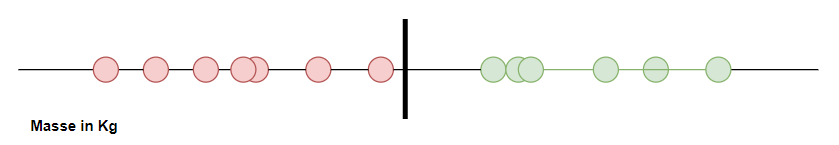
\includegraphics[width=10.0cm]{pic/SVC_1D.png}
    \caption{Beispiel eines Support Vector Classifiers}
    \label{fig:SVC_1D}
\end{figure}

In Abb. \ref{fig:SVC_1D} ist der SVC ein Punkt auf einer eindimensionalen Linie, auf der das Gewicht in Kg von z.B. 
Mäusen in ,,Unter-'' und ,,Übergewichtig'' unterteilt wird. Dieser Punkt ist Ergebnis aller Verhältnisse der einzelnen
Datenpunkte zueinander. Durch sog. ,,\textit{Kernel Funktionen}'' versucht der Algorithmus nun Beziehungen 
in höheren Dimensionen zu finden, wie z.B. $Masse^2$, $Masse^3$ usw. . Der SVC stellt dann in diesen Dimensionen 
eine Linie in einem zwei-dimensionalen oder eine Ebene in einem drei-dimensionalen Koordinatensystem dar.\\

\begin{figure}[h]
    \centering
    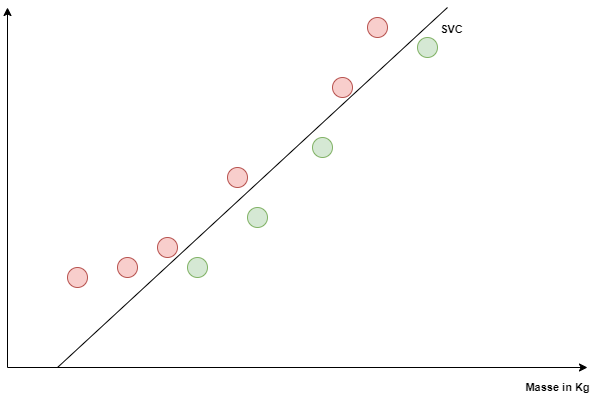
\includegraphics[width=10.0cm]{pic/SVC_2D.png}
    \caption{Beispiel eines Support Vector Classifiers in der zweiten Dimension}
    \label{fig:SVC_2D}
\end{figure}

Da der SVC die Verhältnisse aller Datenpunkte zueinander betrachtet, ist er sehr anfällig für Ausreißer in 
den Daten, was bei der Datenvorbereitung und der Auswertung beachtet werden muss.

\newpage
\subsection{Logistische Regression}

Die logistische Regression ordnet Daten einem bestimmten Label anhand einer Wahrscheinlichkeit zu. Trotz dem Teilnamen
,,Regression'' handelt es sich um einen Klassifizierungsalgorithmus. Der Name kommt daher, dass die berechnete Wahrscheinlichkeit
zu einem kontinuierlichen Label zwischen 0 und 1 führt, was durch die Form einer Sigmoid-Funktion ausgedrückt wird.
Der Algorithmus eignet sich wegen dieser Eigenschaft besonders für  das Klassifizierungsproblem der Projektarbeit, 
bei der ein Wahrheitswert, wie ,,Anwesenheit'' oder ,,Abwesenheit'' untersucht werden soll.\\
Nutzt man logistische Regression beispielsweise zur Abbildung einer Beziehung zwischen Gewicht von Mäusen in Gramm 
zu einer Wahrscheinlichkeit für Übergewicht, könnte das entstehende Modell wie folgt aussehen.

\begin{figure}[h]
    \centering
    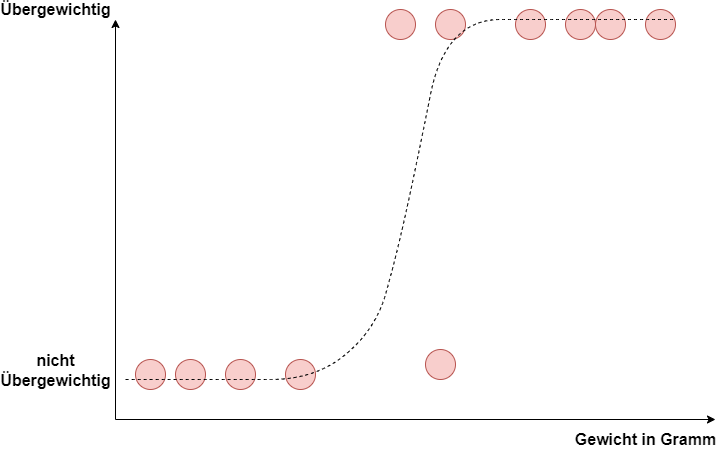
\includegraphics[width=10.0cm]{pic/logistic_regression.png}
    \caption{Beispiel logistischer Regression}
    \label{fig:SVC_2D}
\end{figure}

Die Sigmoid-Funktion wird grundsätzlich durch

\begin{align}
    p = \frac{1}{1 + e^{-(x-\mu)/s}}
\end{align}

beschrieben, wobei x der Eingabewert in Gramm und $\mu$ der Mittelpunkt der Kurve beschreibt, der sich aus dem 
Verhältnis von Eintrittswahrscheinlichkeit $p_1$ und Gegenwahrscheinlichkeit $p_0$ ergibt.

\begin{align}
    p(\mu) = 0.5 = \frac{p_1}{p_0}   
\end{align}

\newpage
Zusätzlich beschreibt s einen Skalierungsparameter, mit dem die Form der Kurve flacher oder steiler werden kann,
was angibt, wie eindeutig die hereingegebenen Daten zugeordnet werden können. Wären im o.g. Beispiel also alle roten
Punkte jeweils links und rechts von der Mitte einsortiert, wäre die Sigmoid-Funktion in der Mitte sehr steil, da alle
Daten anhand des Mittelpunktes klar getrennt werden könnten.

\begin{figure}[h]
    \centering
    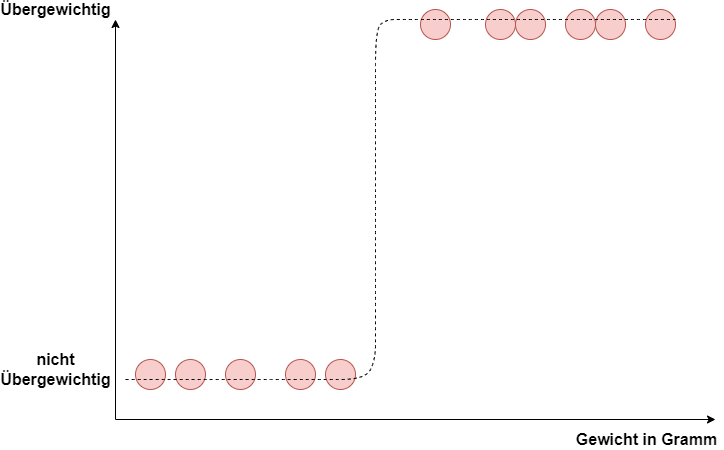
\includegraphics[width=10.0cm]{pic/logistic_regression_high s.png}
    \caption{Logistische Regression mit deutlicher Skalierung}
    \label{fig:SVC_2D}
\end{figure}

Anhand der optimierten Sigmoid-Funktion können nun neue Daten klassifiziert werden, wobei die Wahrscheinlichkeit
bei $p < 0.5$ auf 0 und $p >= 0.5$ auf 1 gerundet wird.
\newpage
\subsection{K-Nearest-Neighbours}
Der \textit{K-Nearest-Neighbours}-Algorithmus KNN betrachtet den Abstand von einem gegebenen Punkt $p$ zu einer 
Menge an Punken in einem Datenset und ordnet ihn gemäß dieser Abstände einer bestimmten Kategorie zu. Die 
Zuordnung geschiet anhand der Kategorie der größten Menge an nähesten Nachbarn.

\begin{figure}[h]
    \centering
    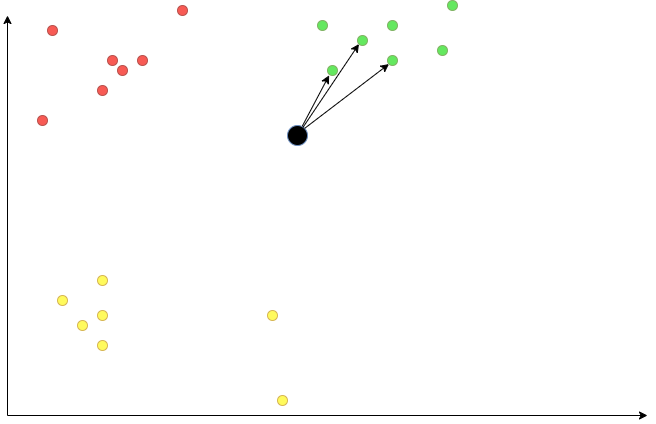
\includegraphics[width=12.0cm]{pic/KNN.png}
    \caption{Beispiel eines KNN}
    \label{fig:NN}
\end{figure}

Im oben gezeigten Beispiel würde ein Punkt anhand seiner drei nächsten Nachbarn als "grün" kategorisiert.
Die Anzahl der gewünschten Nachbarn die zu untersuchen sind, ist frei wählbar.
Da die Abstandsberechnung über den \textit{Euklidischen Abstand} berechnet wird, funktioniert dieser 
Algorithmus auch in höheren Dimensionen, da 

\begin{align}
    d = \sqrt{(x2 - x1)^2 + (y2 - y1)^2 + (z2 - z1)^2 + ... + (n2 - n1)^2}
\end{align}

sich in beliebig viele Dimensionen fortsetzen lässt.
\newpage
\subsection{Neuronale Netzwerke}
Die Funktionsweise eines Neuronalen Netzwerks ist direkt angelehnt an die Funktionsweise des menschlichen Gehirns.
Einzelne Knotenpunkten(Neuronen) werden mithilfe von Gewichteten Verbindungen verknüpft, sodass das Netzwerk versucht 
Eingabewerte bestimmten Ausgabewerten zuzuordnen. Diese Zuordnung der Ein- und Ausgabewerte im Input- und Output-Layer 
geschiet nicht direkt, sondern durch ein oder mehrere \textit{Hidden Layer}, dessen Neuronenzahl üblicherweise über 
der Anzahl Neuronen im Input Layer liegt. Die Anzahl der Neuronen im Output-Layer entspricht der Anzahl an Ergebnissen, 
die sich aus dem Input Ergeben können. Im Beispiel der Anwesenheitsanalyse entspräche das hier also zwei Neuronen für 
An- und Abwesenheit.

\begin{figure}[h]
    \centering
    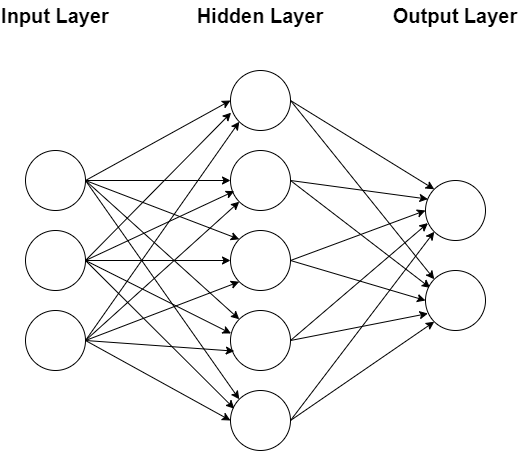
\includegraphics[width=10.0cm]{pic/NN.png}
    \caption{Beispiel eines neuronalen Netzwerks}
    \label{fig:NN}
\end{figure}

Liegt an einem Neuron eine Information an, wird diese als Eingabe einer Aktivierungsfunktion $\varphi$ genutzt, 
die mithilfe eines bestimmten Schwellwertes bestimmt, ob dieses Neuron aufgrund der Eingabe aktiviert wird. Über eine 
bestimmte Anzahl von Iterationen werden die Gewichtungen zwischen den einzelnen Neuronen stärker oder schwächer.


\subsection{Long Short Term Memory}
Das \textit{Long Short Term Memory} LSTM ist eine Abwandlung herkömmlicher Neuronalen Netzwerke. Es handelt sich um ein
\textit{rekurrentes} Neurales Netzwerk, was bedeutet, dass jedes Neuron seine Ausgabewerte auch wieder als Eingabewerte
nutzt. Der Begriff \textit{Memory} rührt daher, dass durch diese Rückkopplung eine Art Gedächtnis entsteht, durch 
die das Netzwerk bessere Rückschlüsse auf die Einordnung des aktuellen Input-Wertes ziehen kann.\\

\begin{figure}[h]
    \centering
    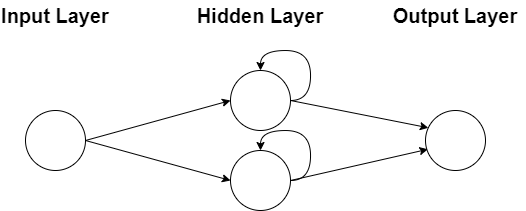
\includegraphics[width=10.0cm]{pic/RecurrentNN.png}
    \caption{Beispiel eines rekurrenten neuronalen Netzwerks}
    \label{fig:RecNN}
\end{figure}
\newpage
Bei einem LSTM verfügt jedes Neuron zusätzlich über einen Zell-Status $C_t$, welcher durch einen Input $x_t$ verändert werden kann.
Auf den Zell-Status nehmen \textit{Input-}, \textit{Forget-} und \textit{Output}-Gates Einfluss. Diese drei Gates
besitzen jeweils ein eigenes neronales Netzwerk $\sigma$.\\\\
Das Input-Gate bestimmt, ob der Zell-Status anhand des anliegenden Inputs verändert werden darf.
Das Forget-Gate gibt an, ob der Status der Zelle zurückgesetzt und somit das ,,Gedächtnis'' der Zelle gelöscht wird. Es
stellt die zentrale Komponente des LSTMs dar.
Das Output-Gate regelt, ähnlich wie Aktivierungsfunktion normaler NNs, ob der anliegende Input zu einem Output 
der Zelle führt.

\begin{figure}[h]
    \centering
    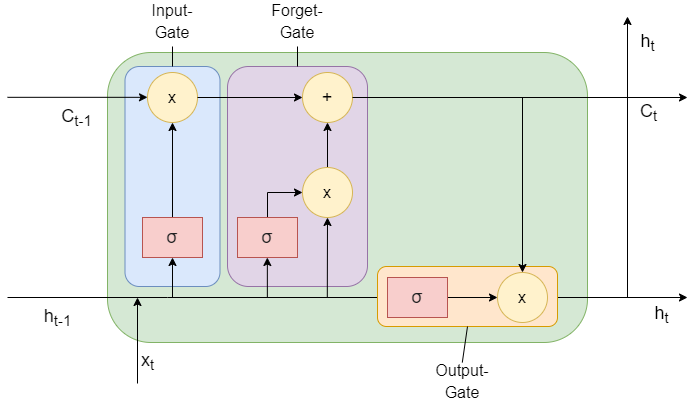
\includegraphics[width=12.0cm]{pic/LSTM-Cell.png}
    \caption{Vereinfachter Aufbau einer LSTM-Zelle}
    \label{fig:RecNN}
\end{figure}

Ein LSTM kann auf diese Weise eine Vielzahl von Zeitschritten zurückblicken und verlässt sich so nicht direkt auf 
einen gegebenen Input, sondern auf einen langen Verlauf von bereits verarbeiteten Input-Werten. 
LSTMs sind deshalb besonders interessant für Probleme bei denen Beziehungen zwischen kontinuierlichen 
Datenwerten gebildet werden müssen.

\newpage
Geht man von einem LSTM aus, dass über eine Liste an Namen verfügt und anhand einem Datensatz gelernt
hat, zwei Namen mit der Beziehung ,,sah'' zu z.B. ,,Jonas sah Jakob.'' zu verknüpfen.\\
Das LSTM hat nun intern einen Status, der angibt, dass auf einen Namen mit hoher Wahrscheinlichkeit das Wort 
,,sah'' und mit niedriger Wahrscheinlichkeit ein zweiter Name folgt. 
Beginnt man nun einen neuen Satz mit ,,Jakob'', werden als mögliche nächste Worte ,,Jonas'', ,,Jakob'' und ,,sah''
ausgewählt. Bisher ähnelt dieser Verlauf einem normalen Neuronalen Netzwerks. Beim LSTM
steht aber nun wegen dem vorherigen Durchlauf der Name ,,Jakob'' im Forget-Gate, sodass ,,Jakob'' aus der verfügbaren
Wortauswahl für das nächste Wort gelöscht wird.\\



\section{CO2 als Anwesenheitsindikator}\label{CO2}

%Der CO2-Gehalt der Raumluft ist als sehr guter Indikator für menschliche Präsenz anzusehen. Anders als andere 
%Umweltindikatoren wie Temperatur oder Luftfeuchtigkeit hat der CO2-Gehalt die Eigenschaft, dass es in 
%geschlossenen Räumen keine äußeren Einflussfaktoren für diesen Messwert gibt. In einem Büroraum kann der 
%Mensch als alleinige Quelle für CO2 angesehen werden.\\
Der Anteil von CO2 in frischer Atemluft beträgt zwischen 350 und 450 ppm. Es gibt in Deutschland und auch Europa 
keine grundsätzlich festgelegten Grenzwerte für akzeptable Raumluft, vielmehr raten Gesundheitsämter 
verschiedener Länder Grenzwerte zwischen 1200 und 1500 ppm einzuhalten. Bei der Obergrenze von 1500 ppm 
entstehen beim Menschen erste Müdigkeitserscheinungen, weshalb dieser Wert in der Literatur als maximaler 
Richtwert für Innenräume gilt.\\

\begin{figure}[h]
    \centering
    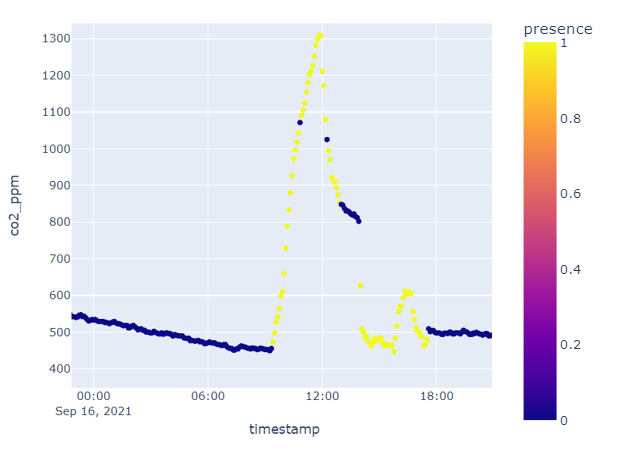
\includegraphics[width=0.7\textwidth]{pic/co2_singleDay.png}
    \caption{CO2 Gehalt der Raumluft über einen Tag}
    \label{fig:CO2_oneDay}
\end{figure}
 
Es ist zu erkennen, dass die CO2-Werte in einem normalen Büroraum innerhalb dieser empfohlenen Grenzen schwanken.
Mit einigen kleinen Pausen sind fast durchgehend Personen anwesend, die täglich etwa um 12:00 den Raum lüften.
Es ist auch klar zu erkennen, dass sich der CO2-Gehalt während Abwesenheit durch die passive Lüftung des Raumes  
(Tür-/Fensterspalten) langsam wieder gegen den Grundwert bewegt.

\newpage
\section{Luftfeuchtigkeit und Temperatur}
Auch wenn Luftfeuchtigkeit und Temperatur Indikatoren für menschliche Präsenz in einem Raum sein können, 
unterliegen sie in ihrer Nützlichkeit dem CO2-Gehalt der Raumluft in einem wichtigen Faktor. 
Sie sich beide stark beeinlusst, von äußeren Umweltfaktoren wie dem aktuellen Wetter oder der Jahreszeit.
Beide Werte wurden zunächst in das Training aller Modelle miteinbezogen, es wird allerdings im Folgenden 
Kapitel gezeigt, dass diese beiden Werte zusammen mit dem CO2-Werte nicht von besonderem Nutzen sind und 
deshalb später nicht weiter genutzt werden.  

\section{Sensordaten}
Wie bereits beschrieben, wurden die Sensordaten in mehreren Räumen der FH Aachen kontinuierlich 
gesammelt. Durch das Filtern nach der Beziehung des Raumes ergab sich folgende Datenstruktur als
Ausgangslage:\\

\begin{tabular}{|p{4.5cm}||p{3cm}|p{7cm}|}
    \hline
    \multicolumn{3}{|c|}{Sensordaten} \\
    \hline
    Name&Format &Beschreibung\\
    \hline
    timestamp&timestamp&Zeitpunkt der Messung\\
    co2\_ppm&integer&CO2-Wert\\
    temperature\_celsius&float&Temperatur in Grad Celsius\\
    relative\_humidity\_percent&float&Luftfeuchtigkeit\\
    presence&boolean&Aktivität des Bewegungssensors\\
    \hline
\end{tabular}     

\chapter{Technische Umsetzung}

\section{Datenbeschaffung und -Vorbereitung}
Die Daten wurden lokal auf einem der FH-Server in Form eines \textit{Hadoop Distributed File System} (HDFS) 
gespeichert. Mithilfe von Apache Drill konnten die Daten jederzeit mit einfachen SQL-Abfragen beschafft werden. 
Die Daten wurden so durch die gesamte Dauer des Projektes immer aktuell gehalten, damit alle Erkenntnisse 
immer auf der aktuellsten Datenlage basieren.
\\\\
Die Datenvorbereitung oder Pre-Processing ist eine der wichtigsten Schritte bei der Anwendung von Machine 
Learning. Durch sie kann man beim Training des Models durch Bearbeitung bestehender Spalten oder Hinzufügen 
von zusätzlichen Spalten im Datenset Schwerpunkte setzen, die es den Algorithmen beim Training zum einen 
erleichtern, ihre Erwartungen zu präzisieren, zum anderen aber auch die Leitung beim Verarbeiten bestimmter 
Spalten zu steigern.
\subsection{Gruppierung}
Die Sensordaten wurden alle sechs Sekunden erfasst. Da sich weder CO2-Gehalt noch Feuchtigkeits- oder 
Temperaturwerte der Raumluft so schnell nicht verändert, wurden die Daten direkt beim Drill per SQL zu 
zwei-Minuten-Intervallen zusammengefasst. Dabei werden über alle Spalten hinweg Durchschnittswerte gebildet, 
die dann nachher zu einem Datensatz zusammengefasst werden. 
Dies steigert die Leistung aller Algorithmen erheblich, da sich die Zahl der 
Datensätze sich stark verringert. Da sich, wie oben erwähnt, der CO2-Gehalt der Raumluft in einem 
Intervall von zwei Minuten kaum merklich verändert, verringert sich die Genauigkeit des gesamten Datensetz 
dadurch nicht maßgeblich.
\subsection{Zyklische Codierung}
Zyklische Codierung wird immer dort verwendet, wo Daten sich in wiederholenden Schemata bewegen. Diese 
Schemata, wie z.B. die Zahlenumbrüche bei einer Uhrzeit, sind für Algorithmen nicht direkt ersichtlich und 
sind zudem für Computer nicht leicht zu verarbeiten. Durch eine Encodierung in 
Sinus- und Cosinus-Werte können diese Zusammenhänge vereinfacht werden.\\
Hierzu wurde der Timestamp zuerst in Sekunden übersetzt, sodass sich ein bestimmter Zeitpunkt eines Tages 
immer zwischen 0 und 86400 Sekunden bewegt.
Aus diesem Wert wurden dann zwei neue Datenspalten ,,\textit{hour\_sin}'' und ,,\textit{hour\_cos}'' 
in das Datenset eingefügt welche sich durch 

\begin{align}
    hour\_sin = sin(2 * \pi * x / x_{max}) \\ 
    hour\_cos = cos(2 * \pi * x / x_{max})
\end{align} 

ergeben. So kann jede Tageszeit einer eindeutigen Kombination aus Sinus- und Cosinus-Werten zwischen 
$0$ und $1$ zugeordnet werden.

\subsection{Deltas und Shift-Werte}
Desweiteren wurden von den Spalten ,,\textit{co2\_ppm}'', ,,\textit{temperature\_celsius}'' und \break 
,,\textit{relative\_humidity\_percent}'', die tatsächlich Rückschlüsse auf die Präsenz zulassen, \break 
zusätzliche Delta- und Shift-Spalten angelegt.\\\\
Ein Shift-Wert bedeutet lediglich, dass  in einer Zeile $x_n$ des Datensets 
zusätzlich, neben den aktuellen Werten, auch Werte von $k$ Zeilen zuvor, also $x_{n-k}$ stehen. So haben 
alle Algorithmen direkten Zugriff auf Vergangenheitswerte der ausgewählten Spalten.\\\\
Delta-Spalten stellen, dem Namen nach, Deltas zu vorherigen Werten dar:

\begin{align}
    \Delta x_k = x_n - x_{n-k}    
\end{align}

Die Erwartung ist hier, dass die Änderung der CO2-, Temperatur- und 
Luftfeuchtigkeitswerte ein wichtigerer Indikator sein könnte, als die tatsächlichen Werte. In einem schlecht 
klimatisierten Raum könnten Grundwerte von z.B. CO2 höher sein, als in anderen Räumen. Durch die hinzufügten 
Deltas werden diese Grundwerte ignoriert und Rückschlüsse auf die aktuelle Präsenz sind besser möglich.\\
Im Zuge der Projektarbeit wurden verschiedene Kombinationsmöglichkeiten von Delta- und Shiftwerten mit 
Zeitschritten zwischen zwei Minuten und einer Stunde mit Hinblick auf Verbesserungen der Model-Genauigkeiten 
getestet.

\subsection{Outlier Detection}
Wie bereits erwähnt, spielen Datenausreißer für die Ergebnisse mancher Algorithmen eine große Rolle. Überall 
wo z.B. aus einer Reihe von Datenwerten Durchschnittswerte berechnet werden, würden Ausreißer in den Daten das 
Ergebnis verfälschen und die Leistung des Algorithmus deutlich senken.
Um diese Ausreißer vor dem Training der Models zu beseitigen wurde das Verfahren des 
\textit{Interquartilabstands} (IQR nach der englischen Bezeichnung \textit{Interquartile Range}) gewählt.\\
Der IQR gibt die Intervallgröße an, die ein Wert vom Median einer Datenreihe abweichen darf. Bei einer 
der Größe nach sortierten Datenreihe $x = (x_0,x_1,...,x_n)$ bestimmt man die Mediane der unteren und oberen 
Hälfe des Datensets $Q_1$ und $Q_2$. Der IQR ergibt sich nun aus 
\begin{align}
    IQR = Q_2 - Q_1
\end{align}
Mit diesm Wert kann man nun die erlaubten Ober- und Untergrenzen 
des Datensets mit 
\begin{align}
    Limit_{upper} = Q_2 + 1.5 * IQR \\
    Limit_{lower} = Q_1 - 1.5 * IQR
\end{align} 
bestimmen. Alle Werte die außerhalb dieser Grenzen liegen, können als Ausreißer betrachtet werden.\\
Ausreißer zu entfernen, ist hier wichtig, da die Sensoren Messfehler erzeugen können, oder gelegentlich zur 
Demonstration von starken Veränderungen in der direkten Nähe des Sensors geatmet wurde und es so in vielen 
Datensets kurzfristige CO2-Werte gibt, die natürlich in geschlossenen Räumen nicht vorkommen.

\section{Validierung}
\sloppy
Über das Projekt hinweg wurden verschiedene Validierungsmethoden verwendet. Grundsätzlich unterteilt man das 
Datenset in ein Trainings- und Testset mit einem Verhältnis von etwa 80-20. Das bedeutet, dass das Model mit
80 prozent der Daten trainiert wird, wobei die anderen 20 prozent zurückgehalten werden, um daraufhin das 
fertig trainierte Model daran zu testen. Aus dem Ergebnis dieses Tests ergeben sich verschiedene Werte, die  
die allgemeine Genauigkeit des Models repräsentieren, d.h. wie verlässlich das Model die An- und Abwesenheit 
des Testsets selbst berechnen kann, wenn man ihm den tatsächlichen Wert vorenthält.\\
Allgemeine Basis für die errechneten Genauigkeiten bildet die sog. \textit{Confusion Matrix}.

\begin{figure}[h]
    \centering
    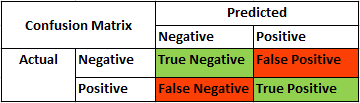
\includegraphics[width=0.6\textwidth]{pic/confusion_matrix_ex.png}
    \caption{Beispiel einer Confusion Matrix}
    \label{fig:CV}
\end{figure}

Diese zeigt, inwiefern sich die Genauigkeit des Modells neben tatsächlich richtig erkannten Werten zusätzliche
aus false negatives und false positives zusammensetzt.\\
\newpage
Die \textit{Accuracy Score} ist eine einfache Methode zur Bestimmung der Modellqualität und berechnet sich 
aus der Summe der richtigen Ergebnisse geteilt durch die Summe aller Ergebnisse.

\begin{center}
    $AccuracyScore = \dfrac{TP + TN}{TP + TN + FP + FN}$    
\end{center}
Die \textit{Recall Score} beschreibt die Genauigkeit bezogen auf alle erkannten positiven Ergebniswerte. 
%Dabei ist wichtig, dass wenn ein Algorithmus beispielsweise Anwesenheit zu erkennen versucht auch ein
%false negative als Treffer gewertet wird.
\begin{center}
    $RecallScore = \dfrac{TP}{TP + FN}$    
\end{center}

Die \textit{Precision Score} gibt die allgemeine Menge, an positiven Werten, die hätten erkannt werden müssen,
an.
\begin{center}
    $PrecisionScore = \dfrac{TP}{TP + FP}$    
\end{center}

Die \textit{F1-Score} ist der Durchschnittswert aus Recall- und Precision-Score und gibt im Allgemeinen eine 
gute Auskunft über die Qualität eines Modells.\\

\begin{center}
    $F1\_Score = \dfrac{2}{\dfrac{1}{PrecisionScore} + \dfrac{1}{RecallScore}} = \dfrac{2 \cdot (PrecisionScore \cdot RecallScore)}{PrecisionScore + RecallScore}$    
\end{center}

\vspace{0.75cm}
In diesem Anwendungsfall ist es durchaus wichtig, Anwesenheitswerte genauer zu betrachten als 
Abwesenheitswerte, da ein Arbeitstag nur etwa ein Drittel eines tatsächlichen Tages darstellt. 
Das Datenset ist also mit einem Verhältnis von etwa 8/16 in Richtung der Abwesenheit unausgeglichen. Dies 
lässt die Erwartung zu, dass das trainierte Model wesentlich besser darin sein wird, Abwesenheit zu erkennen,
als Anwesenheit.\\
Hierzu wurde bei der Auswertung der Ergebnisse immer auch der \textit{Classification Report} hinzugezogen,
aus dem ersichtlich ist, wie genau das Model beide möglichen Labelwerte berrechnen konnte.
\newpage
Desweiteren war es entscheidend zu erkennen, dass das Datenset über mehrere Monate hinweg nicht perfekt uniform 
ist, da es in bestimmten Monaten zu verhätlnismäßig vielen Urlaubstagen (z.B. Weihnachten/Silvester) und damit 
einer Häufung an Abwesenheits-Werten kommt.
Wenn die Daten nun im o.g. Verhältnis aufgeteilt werden und dann viele Daten des Testsets in solchen Monaten 
liegen, könnte es beim Ergebnis zu Verzerrungen kommen.\\
Hierfür wurde eine \textit{Kreuzvalidierung} (engl. Cross Validation CV) implementiert. Bei einer CV wird das 
Datenset immernoch im gleichen Verhältnis aufgeteilt, allerdings mehrmals, sodass die Trainings- und Testsets 
jedes mal aus jeweils anderen Daten bestehen.

\begin{figure}[h]
    \centering
    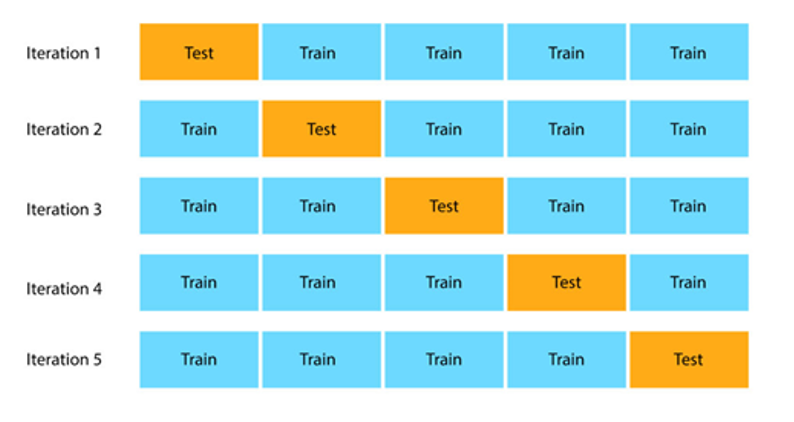
\includegraphics[width=0.7\textwidth]{pic/CV.png}
    \caption{Beispiel einer Kreuzvalidierung}
    \label{fig:CV}
\end{figure}

Errechnet man nun die Durchschnittsgenauigkeit aller Iterationen der CV, ergibt sich eine Gesamtgenauigkeit, 
die das Model besser repräsentiert, weil es an einer größeren Anzahl an verschiedenen Daten trainiert und 
getestet wurde.
\\\\
Da es für manche Räume keine Datensätze mit Labelwerten gab, musste die Validierung dieser Datensätze 
augenscheinlich erfolgen. Hierfür wurde in ein Datenset eine Labelspalte eingefügt, die dann vom trainierten
Model selbst gefüllt werden sollte. Das Ergebnis musste dann in einem Graphen gezeichnet und per Hand validiert 
werden. Da sich das Ergebnis der Berechnung in diesem Anwendungsfall, wie oben gezeigt, sehr übersichtlich als 
Graph darstellen lässt, war diese Methode der Validierung zwar nicht perfekt, lieferte aber trotzdem einen 
ausreichenden Eindruck über die Qualität des trainierten Models.


\subsection{Over- und Underfitting}
Over- und Underfitting sind Probleme, die bei allen Machine Learning Algorithmen auftreten können und bezeichnen 
im Allgemeinen einen falschen Umgang mit dem Datenset.
\textit{Overfitting} bedeutet, dass das Modell mit zu vielen, sich zu stark ähnelnden, Daten trainiert wurde, 
wodurch es nur in der Lage ist, neue Daten richtig zu kategorisieren, die dem Trainingsset besonders ähnlich sind.
Overfitting kann während einer Kreuzvalidierung oder Validierung anhand eines anderen Datensets, als dem 
Trainingsset, erkannt werden.\\
Um Overfitting zu verhindern, kann das Datenset zu vereinfacht werden, um so die Beziehungen zwischen den
für die Erwartungsberechnung relevanten Spalten zu stärken.\\\\
\textit{Underfitting} bedeutet dagegen, dass es das Modell nicht geschafft hat, zwischen den gegebenen Daten
Beziehungen herzustellen, die das Modell unbekannte Daten richtig kategorisieren lassen. Hier reicht es 
normalerweise aus, dem Modell mehr Daten zur Verfügung zu stellen und in der Datenvorbereitung Felder 
einzufügen, die dem Modell bestimmte Beziehungen zwischen Datenfeldern hervorheben sollen. 

\subsection{Parameter Tuning}
\textit{Parameter Tuning} beschreibt einen Schritt der Modell-Optimierung, der normalerweise stattfindet, 
nachdem ein funktionierendes Modell, das mit bereits verarbeiteten Daten gute Ergebnisse liefert, erstellt 
wurde. Jedes Modell besitzt Parameter, die bei der Erstellung festgesetzt werden. Diese Parameter haben 
großen Einfluss auf den Trainingsprozess, weshalb es sich anbietet, die Genauigkeiten mehrerer Modelle 
mit verschiedenen Paramter-Kombinationen zu testen.\\
Das im Scikit-Learn enthaltene \textit{GridSearchCV}-Modul
bietet die Möglichkeit einem Modell eine Vielzahl an verschiedenen Parameter-Optionen zu übergeben. Mit diesen 
werden kann automatisch Modelle trainiert und per Kreuzvalidierung verglichen. Am Ende liefert das Modul 
die Parameter-Kombination, mit der das beste Ergebnis erzielt wurde.

\begin{figure}[h]
    \centering
    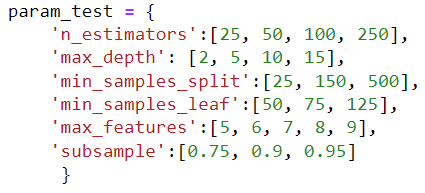
\includegraphics[width=0.6\textwidth]{pic/param_test.png}
    \caption{Beispiel einer Sammlung von Parameter-Optionen}
    \label{fig:CV}
\end{figure}

Im obenstehenden Beispiel kann man erkennen, dass für bestimmte Parameter (rot) eine Sammlung an erlaubten 
Werten (grün) übergeben werden. Alle Kombinationen aus diesen Parameter-Optionen werden dann vom 
GridSearchCV-Modul ausgewertet.\\
Die Verbesserungen gegenüber Standard-Parametern bewegen sich normalerweise im niedrigen einstelligen 
Prozent-Bereich und kann auch zu einer leichten Verschlechterung führen, wenn die Standard-Parameter
der einzelnen Modelle bereits gut gewählt waren.
%% Zwei Abbildungen, die zusammen gehören

%\begin{figure}
%        \centering
%        \begin{minipage}[c]{0.45\textwidth}
%                \includegraphics[height=6.5cm]{pic/dateiname1.png}
%        \end{minipage}
%        \begin{minipage}[c]{0.45\textwidth}
%                \includegraphics[height=6.5cm]{pic/dateiname2.png}
%        \end{minipage}
%        \caption{Zwei Abbildungen}\label{fig:zwei_abb}
%\end{figure}
